\documentclass[12pt, titlepage]{article}

\usepackage{fullpage}
\usepackage[round]{natbib}
\usepackage{multirow}
\usepackage{booktabs}
\usepackage{tabularx}
\usepackage{graphicx}
\graphicspath{ {./images/} }
\usepackage{float}
\usepackage{hyperref}
\hypersetup{
    colorlinks,
    citecolor=blue,
    filecolor=black,
    linkcolor=red,
    urlcolor=blue
}

%% Comments

\usepackage{color}

\newif\ifcomments\commentstrue %displays comments
%\newif\ifcomments\commentsfalse %so that comments do not display

\ifcomments
\newcommand{\authornote}[3]{\textcolor{#1}{[#3 ---#2]}}
\newcommand{\todo}[1]{\textcolor{red}{[TODO: #1]}}
\else
\newcommand{\authornote}[3]{}
\newcommand{\todo}[1]{}
\fi

\newcommand{\wss}[1]{\authornote{blue}{SS}{#1}} 
\newcommand{\plt}[1]{\authornote{magenta}{TPLT}{#1}} %For explanation of the template
\newcommand{\an}[1]{\authornote{cyan}{Author}{#1}}

%% Common Parts

\newcommand{\progname}{ProgName} % PUT YOUR PROGRAM NAME HERE
\newcommand{\authname}{Team \#, Team Name
\\ Student 1 name
\\ Student 2 name
\\ Student 3 name
\\ Student 4 name} % AUTHOR NAMES                  

\usepackage{hyperref}
    \hypersetup{colorlinks=true, linkcolor=blue, citecolor=blue, filecolor=blue,
                urlcolor=blue, unicode=false}
    \urlstyle{same}
                                


\newcounter{acnum}
\newcommand{\actheacnum}{AC\theacnum}
\newcommand{\acref}[1]{AC\ref{#1}}

\newcounter{ucnum}
\newcommand{\uctheucnum}{UC\theucnum}
\newcommand{\uref}[1]{UC\ref{#1}}

\newcounter{mnum}
\newcommand{\mthemnum}{M\themnum}
\newcommand{\mref}[1]{M\ref{#1}}

\begin{document}

\title{System Design for Pot-pulator} 
\author{Team \#24, The Nursery Project\\Aaron Billones, billonea\\Gillian Ford, fordg\\Juan Moncada, moncadaj\\Steven Ramundi, ramundis}
\date{January 18, 2023}

\maketitle

\pagenumbering{roman}

\section{Revision History}

\begin{tabularx}{\textwidth}{p{3cm}p{4cm}X}
  \toprule {\bf Date} & {\bf Version} & {\bf Notes}\\
  \midrule
  2023-01-18 & Juan Moncada,& Initial release\\&Aaron Billones,\\&Steven Ramundi,\\&Gillian Ford \\
  
  \bottomrule
  \end{tabularx}

\newpage

\section{Reference Material}

This section records information for easy reference.

\subsection{Abbreviations and Acronyms}

\renewcommand{\arraystretch}{1.2}
\begin{tabular}{l l} 
  \toprule		
  \textbf{symbol} & \textbf{description}\\
  \midrule 
  \progname & Explanation of program name\\
  \wss{...} & \wss{...}\\
  \bottomrule
\end{tabular}\\

\newpage

\tableofcontents

\newpage

\listoftables

\listoffigures

\newpage

\pagenumbering{arabic}

\section{Introduction}

The Pot-pulator is a machine with purpose of aiding Sheridan Nurseries in 
populating their trays with pots, in order to prepare them for filling with 
soil and seeds.\\\\Their current method of populating the trays with pots is a 
process with little to no automation, requiring many manual hours of labour. 
Each year, 250,000 annual plants need to be produced by the nursery. Recently, 
the supervisors have found it increasingly more difficult to fill positions with 
enough workers to run the operation smoothly and meet production demand. 
The Pot-pulator will alleviate the large reliance on manual labour and 
improve the overall efficiency of the nursery. \\\\This document consists of a 
detailed design overview of the Pot-pulator. The system overview, system 
variables, user interfaces, hardware design and electrical design will be 
presented in this document.


\section{Purpose}

This document describes the overall system functionality and the design overview 
of the Pot-pulator. It will describe how the mechanical, electrical, and software 
components will interact with each other, and the various design decisions made 
within the system. The Module Guide (MG) and Module Interface Specification (MIS) 
are additional design documents that provide a further in depth design of the 
components in each module of the system.

\section{Scope}
The following figure shows the boundary between the Pot-pulator device and its functionality
within the given environment.

\begin{figure}[H]
  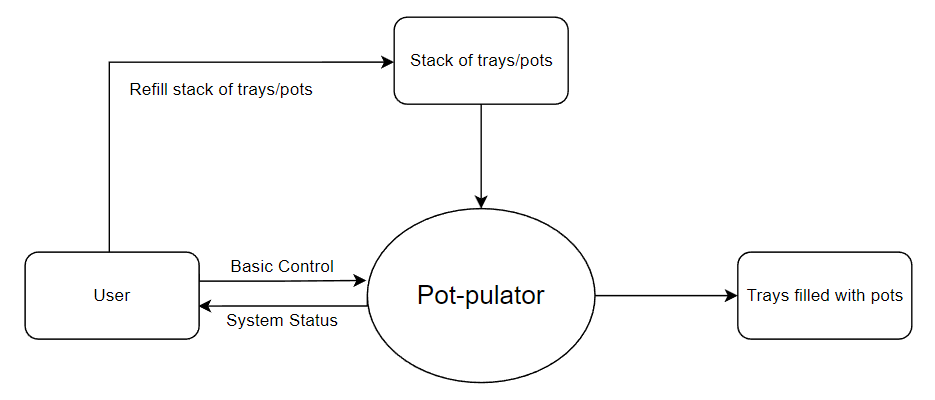
\includegraphics[width=\linewidth]{scope.PNG}
  \caption{System Context Diagram}
  \label{fig:scope}
\end{figure}

\section{Project Overview}

\subsection{Normal Behaviour}

\subsection{Undesired Event Handling}

\wss{How you will approach undesired events}

\subsection{Component Diagram}

\subsection{Connection Between Requirements and Design} \label{SecConnection}

\wss{The intention of this section is to document decisions that are made
  ``between'' the requirements and the design.  To satisfy some requirements,
  design decisions need to be made.  Rather than make these decisions implicit,
  they are explicitly recorded here.  For instance, if a program has security
  requirements, a specific design decision may be made to satisfy those
  requirements with a password.}

\section{System Variables}

\wss{Include this section for Mechatronics projects}

\subsection{Monitored Variables}

\subsection{Controlled Variables}

\subsection{Constants Variables}

\section{User Interfaces}

\wss{Design of user interface for software and hardware.  Attach an appendix if
needed. Drawings, Sketches, Figma}

The User Interface will consist of a set of buttons to allow the operator to safely 
interact with the machine. It will also consist of audible and visual signals to alert
the operator of any action required (e.g. tray/pot restock, verification error, etc.).
See Appendix A for interface layout concept.

\section{Design of Hardware}

\subsection{Conveyor}

The conveyor subsystem will be comprised of:
\begin{itemize}
  \item 1 conveyor (including belt, motor, gear box and framing)
  \item 1 Arduino Uno microcontroller
  
\end{itemize}
The conveyor has been acquired from Sheridan Nurseries and will not require fabrication.


\subsection{Pot Dropper}

The pot dropper subsystem will be comprised of:
\begin{itemize}
  \item 4 stepper motors
  \item 4 stepper motor drivers
  \item 1 Arduino Uno microcontroller
  \item 4 pot dropper screws
  \item 1 ultrasonic range finder
\end{itemize}
The pot dropper will be fabricated with steel x-beam framing to support the mechanism.
See Appendix B.1 for a CAD diagram of the pot dropper screw.

\subsection{Tray Dropper}

The tray dropper subsystem will be comprised of:
\begin{itemize}
  \item 2 stepper motors
  \item 1 Sanguinololu driver board
  \item 2 belts
  \item 4 belt bearings
  \item 1 steel x-beam frame
  \item 1 tray dropper end-effector
\end{itemize}
The tray dropper will be fabricated with x-beam framing to support the mechanism. The 
stepper motors and belt bearings will be attached to the framing, and the belts will 
be secured to the bearings. See Appendix B.2 for a CAD diagram of the tray dropper 
end-effector.

\subsection{Tray Elevator}

The tray elevator will be comprised of:
\begin{itemize}
  \item 4 L-shaped wood frame supports
  \item 4 long wood frame supports
  \item 4 short wood frame supports
  \item 1 wood raising platform
  \item 1 ultrasonic range finder
  \item 2 spur gears
  \item 2 racks
  \item 2 stepper motors
\end{itemize}
The wooden frame will be fabricated with screws and wood glue. The stepper motors 
will be attached to either side of the wood platform responsible for hodling the 
stack of trays. The spur gears will be attached to the stepper motors. The racks 
will be attached in the centre of the long wood supports on either side of the frame, 
and will mesh with the spur gears. This will enable the stepper motors to control the 
lifting and lowering of the tray elevator based on its current capacity (see Appendix B.3
for CAD diagram).

\subsection{Verification}

The verification subsystem will be comprised of:
\begin{itemize}
  \item 2 ultrasonic range finders
\end{itemize}

\section{Design of Electrical Components}

The Pot-pulator has a number of electrical components in the system. A complete overview of the circuit diagram
can be found in section C of the appendix. To improve modularity and for easier troubleshooting,
the electrical components were divided in to 4 subsystems based on the control of the system: conveyor control, pot
control, tray control, and verification. These subsystems are each controlled using an 
Arduino Uno while being monitored by the main microcontroller (STM32F429I-DISC1). For each subsystem,
its respective Arduino controls the motors and reads sensor/switch/button values in order to ensure smooth operation. 
The Arduino relays the operation status to the STM32F429I-DISC1 via status bits, that are sent from each of the 
subsystems to the STM32F429I-DISC1 at all times. If an error were to occur in
one of the subsystems, the STM32F429I-DISC1 will be notified and tell all other subsystems to pause operation.



\section{Design of Communication Protocols}

\wss{If appropriate}

\section{Timeline}

\wss{Schedule of tasks and who is responsible}

% \bibliographystyle {plainnat}
% \bibliography{../../../refs/References}

\newpage{}

\appendix

\section{Interface}

% \wss{Include additional information related to the appearance of, and
% interaction with, the user interface}

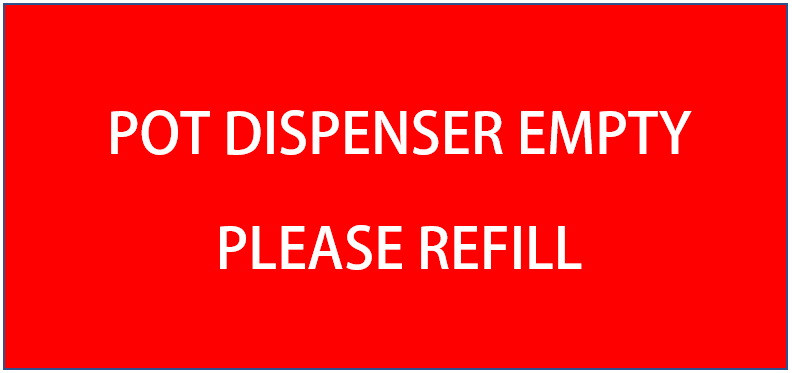
\includegraphics{interface1.png}
\newline
An example of a status message alerting the machine operator that the pot 
dispenser requires refill. This would be accompanied by an audible alert.

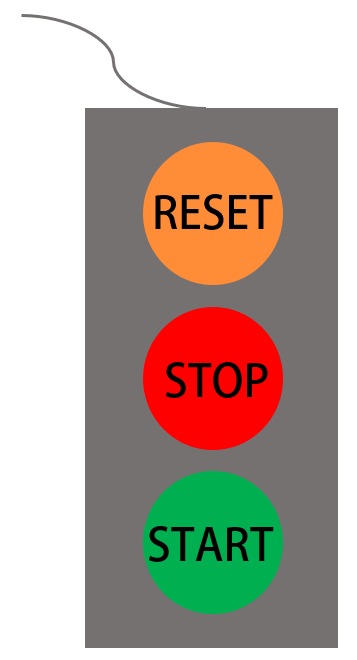
\includegraphics{interface2.png}
\newline
Concept of the button interface used by the operator to control the machine. 
Handheld as to mitigate any safety concerns with a machine-mounted apparatus.

\section{Mechanical Hardware}

\subsection{Pot Dropper}

\subsection{Tray Dropper}

\subsection{Tray Elevator}
\begin{figure}[H]
  \centering
  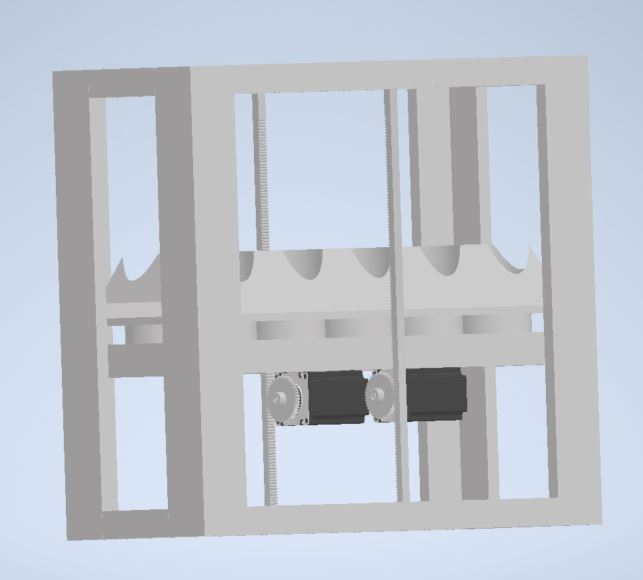
\includegraphics{Tray_Elevator.jpg}
  \caption{Tray Elevator (side)}
  \label{fig:elevator1}
\end{figure}

\begin{figure}[H]
  \centering
  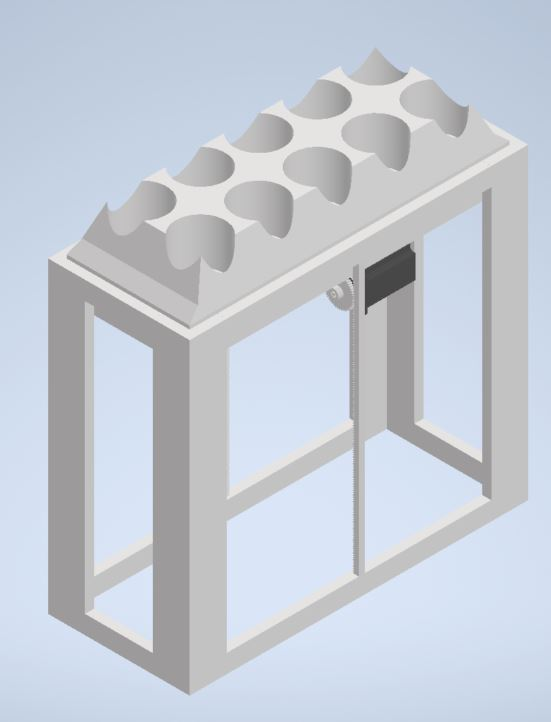
\includegraphics{Tray_Elevator2.jpg}
  \caption{Tray Elevator (orthographic projection)}
  \label{fig:elevator2}
\end{figure}

\section{Electrical Components}

\begin{figure}[H]
  \centering
  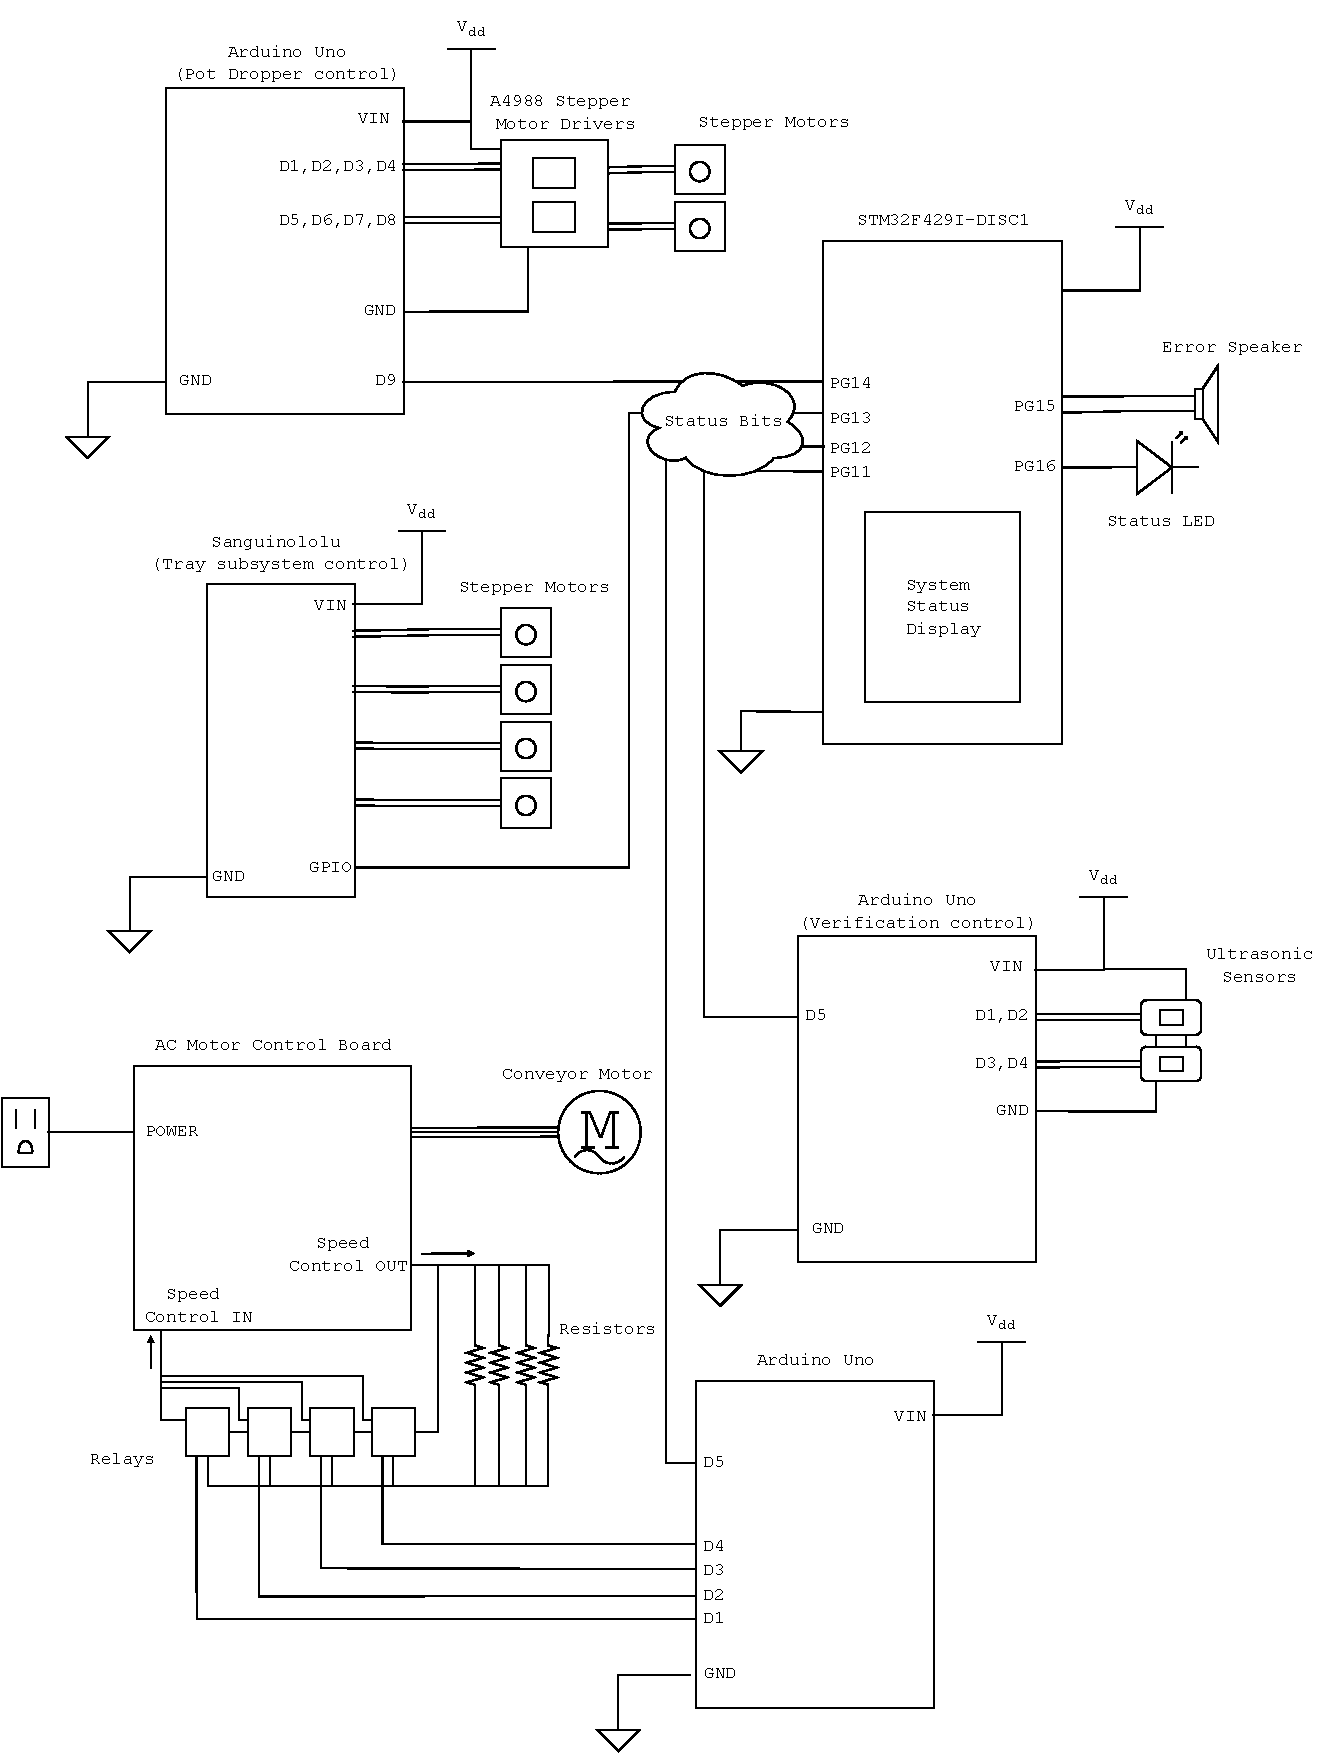
\includegraphics[width=0.89\textwidth]{circuit_diagram.pdf}
  \caption{Circuit Diagram}
  \label{fig:circuit}
\end{figure}

\section{Communication Protocols}

\section{Reflection}

The information in this section will be used to evaluate the team members on the
graduate attribute of Problem Analysis and Design.  Please answer the following questions:

\begin{enumerate}
  \item What are the limitations of your solution?  Put another way, given
  unlimited resources, what could you do to make the project better? (LO\_ProbSolutions)
  \item Give a brief overview of other design solutions you considered.  What
  are the benefits and tradeoffs of those other designs compared with the chosen
  design?  From all the potential options, why did you select documented design?
  (LO\_Explores)
\end{enumerate}

\end{document}